% This is samplepaper.tex, a sample chapter demonstrating the
% LLNCS macro package for Springer Computer Science proceedings;
% Version 2.20 of 2017/10/04
%
\documentclass[runningheads]{llncs}
%
\usepackage{graphicx,wrapfig,xcolor,subfig}
\usepackage{amstext,amsmath,amssymb,bm,bbm,mathtools}
\usepackage{array,multirow}
\usepackage{algorithm2e}


\DeclarePairedDelimiter\norm{\lVert}{\rVert}%
\DeclareMathOperator*{\argmin}{arg\,min}

%% Daniel's definitions
\newcommand{\Ds}{D}
\newcommand{\GG}{ \mathcal{G}_{\vec{I}} }
\newcommand{\GGe}{ \mathcal{G}_{\vec{I}+} }
\newcommand{\GGc}[1]{ \mathcal{G}_C^{(#1)} }
\newcommand{\GGcc}{ \mathcal{G}_C}

\newcommand\figTable[2]{\raisebox{-.5\height}{\includegraphics[scale=#1]{#2}}}

\newcommand\segComparisonGF[2]{figures/segmentation/comparison/#1/#2/alpha-0.0002/beta-1.0/gamma-3.0/radius-7}
\newcommand\segComparisonFF[2]{figures/segmentation/comparison/#1/#2/alpha-0.5/beta-1.0/gamma-3.0/radius-7}
\newcommand\segComparisonScho[2]{figures/segmentation/comparison/#1/lambda-2.0/gamma-1.0/#2}

\begin{document}
%
\title{A maximum-flow model for digital elastica shape optimization}
%
%\titlerunning{Abbreviated paper title}
% If the paper title is too long for the running head, you can set
% an abbreviated paper title here
%
\author{Daniel Martins Antunes\inst{1}\orcidID{0000-0002-6752-0217} \and
Jacques-Olivier Lachaud\inst{1}\orcidID{0000-0003-4236-2133} \and
Hugues Talbot\inst{2}\orcidID{0000-0002-2179-3498}}
%
\authorrunning{D. Martins Antunes et al.}
% First names are abbreviated in the running head.
% If there are more than two authors, 'et al.' is used.
%
\institute{Universit\'e Savoie Mont-Blanc, France
\email{\{daniel.martins-antunes,jacques-olivier.lachaud\}@univ-smb.fr}\\
\and
CentraleSupelec, Universit\'e Paris-Saclay, Inria\\
\email{\{hugues.talbot\}@centralesupelec.fr}}
%
\maketitle              % typeset the header of the contribution
%
\begin{abstract}
  The Elastica is a curve regularization model that integrates the squared curvature in addition to the curve length. It
  has been shown to be useful for contour smoothing and interpolation, for example in the presence of thin
  elements.

  In this article, we propose a graph-cut based model for optimizing the discrete Elastica energy using a fast and
  efficient graph-cut model.  Even thought the Elastica energy is neither convex nor sub-modular, we show that the final
  shape we achieve is often the indeed close to the globally optimal one.

  Our model easily adapts to image segmentation tasks. We show that compared to previous work and state-of-the-art
  algorithm, our proposal is simpler to implement, faster, and yields comparable or better results.

  \keywords{multigrid  convergence \and digital estimators \and curvature \and discrete optimization}
\end{abstract}
%
%
%
\section{Introduction}

The Elastica model and associated energy is a curve regularisation problem with a rich
history~\cite{matsutani2010euler,levien08elastica}, which involves the squared curvature.  It was introduced in computer
vision in~\cite{mumford94elastica} as a means to regularize edges or segmentation boundaries with an explicit curvature
component. Being associated with second-order derivatives, the notion of curvature is difficult to compute and optimize
in a regularisation framework.

Multiple attempts have been made by prominent researchers to introduce an explicit curvature term in curve regularizers
using various methods and approaches. Even early active contour models~\cite{kass88} had an elasticity component
equivalent to a notion of curvature. Similarly, with level-set methods, local curvature can readily be estimated as
in~\cite{malladi1995shape}. However these approches typically optimise a non-convex local energy by gradient descent,
and most were non-geometric, i.e discretization-dependent. In contrast~\cite{caselles97} proposed a geometric level-set
segmentation method, but using only the perimeter as a regularizer, and was still non-convex. All the numerous
approaches based on total-variation minimization for image restoration or segmentation~\cite{rudin1992nonlinear} and
even the Mumford-Shah functional~\cite{mumford89} use this regularization, in part because optimizing it exactly was
already a challenge for a long time~\cite{boykov01fast,chambolle04,appleton2005globally}, either in the discrete or
continuous cases.

In more recent work, optimizing the Elastica, which is a geometric regularizer, has seeen renewed
interest. In~\cite{masnou98inpainting}, authors successfully use a computational geometry approach to perform image
restoration with the Elastica as regularizer. In~\cite{zehiry10fast}, authors compute an approximate discrete version of
the Elastica and optimize it with discrete calculus. In~\cite{nieuwenhuis14efficient}, an efficient, discrete
approximation of curvature is optimized with a specific solver using local submodular
approximations~\cite{gorelick14local}. However, in these works, the quality of the curvature approximation may limit
performance.

In previous work~\cite{antunes2020elastica} we proposed to formulate a digital flow that approximates an
Elastica-related flow using a multigrid-convergent curvature estimator, within a discrete variational
framework. We also presented an application of this model as a post-processing step to a segmentation framework.

In this work, we propose a novel approach that still uses a multigrid-convergent estimation of curvature, that we
optimize using a maximal flow algorithm.

\subsection{Multigrid convergent estimators}
Geometric measurements in digital objects can be tricky.  Intuitively, a good estimator should converge to its
continuous counterpart value as the grid resolution is refined. The criteria that formalizes this intuition is the
multigrid convergence property.

\begin{definition}{(Multigrid convergence)}

  Let $\mathcal{F}$ a family of shapes in the plane and $Q$ a global measurement (e.g., perimeter, area) on members of
  $\mathcal{F}$. Additionally, denote $D_h(S)$ a digitization of shape $S$ in a digital grid of resolution $h$. The
  estimator $\hat{Q}$ of $Q$ is multigrid convergent for the family $\mathcal{F}$ if and only if for every shape
  $S \in \mathcal{F}$, there exists $h_S > 0$ such that
\begin{align*}
\forall h \leq h_S, \quad |\hat{Q}(D_h(S),h) - Q(S)| \leq \tau_S(h),
\end{align*}
%
where $\tau_S:\mathbb{R}_+\setminus \{0\} \rightarrow \mathbb{R}_+$ is the speed of convergence of $\hat{Q}$ towards $Q$
for $S$.
\end{definition}

Tangent and curvature are examples of local properties computed along the boundary of some shape $S$ in the plane. We
need a slight different definition of multigrid convergence in order to map points of the Euclidean boundary to those in
the digital contour.

\begin{definition}{(Multigrid convergence for local geometric quantities)}
  Let $\mathcal{F}$ a family of shapes in the plane and $Q$ a local measurement along the boundary $\partial S$ of
  $S \in \mathcal{F}$. Additionally, denote $D_h(S)$ a digitization of $S$ in a digital grid of resolution $h$ and
  $\partial_h S$ its digital contour. The estimator $\hat{Q}$ of $Q$ is multigrid convergent for the family
  $\mathcal{F}$ if and only if for every shape $S \in \mathcal{F}$, there exists $h_S > 0$ such that the estimate
  $\hat{Q}(D_h(S),p,h)$ is defined for all $p \in \partial_h S$ with $0 < h < h_S$, and for any $x \in \partial S$,
\begin{align*}
	\forall p \in \partial_h S \text{ with } \norm{p-x}_{\infty} \leq h,\quad | \hat{Q}(D_h(S),p,h) - Q(S,x) | \leq \tau_S(h),	
\end{align*}
where $\tau_S:\mathbb{R}_+\setminus \{0\} \rightarrow \mathbb{R}_+$ has null limit at $0$. This function defines the
speed of convergence of $\hat{Q}$ towards $Q$ for $S$.
\end{definition}

We now define the notion of Elastica, particularly in the digital context.

\subsection{Digital Elastica}
The elastica energy of parameters $\vec{\theta}=(\alpha \geq 0, \beta \geq 0)$ for some Euclidean shape
$S \subset \mathbb{R}^2$ is defined as
	\begin{align*}
	E_{\vec{\theta}}(S) &= \int_{\partial S}{ \alpha + \beta \kappa(s)^2 ds}.
	\end{align*}
Similarly, the digital elastica $\hat{E}_{\vec{\theta}}$ of some digitization $D_h(S)$ of $S$ is defined as
	\begin{align}
	\hat{E}_{\vec{\theta}}( D_h(S) ) = \sum_{\dot{\vec{e}} \in \partial_h S}{ \hat{s}( \dot{\vec{e}})\left(\; \alpha + \beta \hat{\kappa}^2(D_h(S),\dot{\vec{e}},h) \; \right)},
	\label{ch5:digital-elastica}
	\end{align}
where $\dot{\vec{e}}$ denotes the center of the linel $\vec{e}$ and the estimators of length $\hat{s}$ and
curvature $\hat{\kappa}$ are multigrid convergent. In the expression above, we will substitute an arbitrary
subset $\Ds$ of $\mathbb{Z}^2$ to $D_h(S)$ since the continuous shape $S$ is unknown.  In the following we omit
the grid step $h$ to simplify expressions (or, putting it differently, we assume that the shape of interest is
rescaled by $1/h$ and we set $h=1$).


\subsection{A multigrid-convergent estimation of curvature}    
Let $S$ be an arbitrary shape. The following definition yields a curvature estimation at every point of its boundary.

\begin{definition}{(Integral Invariant Curvature Estimator)}
  Let $D_h(S)$ a digitization of $S \subset \mathbb{R}^2$. The integral invariant curvature estimator is defined for
  every point $p \in \partial_h S$ as
  \begin{align*}
    \hat{\kappa}_{r}(D_h(S),p,h) \coloneqq \frac{3}{r^3} \left( \frac{\pi r^2}{2} - \widehat{\text{Area}} \left( D_h\big( B_{r} ( p ) \big) \cap D_h(S), h \right) \right).
    %% \hat{\kappa}_{r}(D,x,h) \coloneqq \frac{3}{r^3} \left( \frac{\pi r^2}{2} - \widehat{Area} \left( B_{r/h} ( \frac{1}{h} \cdot x ) \cap D, h \right) \right),
  \end{align*}
\end{definition}
%
where $\widehat{\text{Area}}( D,h )$ estimates the area of $D$ by counting its grid points and then scaling them by
$h^2$. This estimator is multigrid convergent for the family of compact shapes in the plane with $3$-smooth boundary. It
converges with speed $O(h^\frac{1}{3})$ for radii chosen as $r=\Theta(h^\frac{1}{3})$~\cite{lachaud17robust}.


\section{Digital elastica minimization via graph cuts}
In this section we present a graph cut model that converges to the optimum digital shape under digital elastica
regularization. Moreover, the model is easily adapted to image segmentation tasks.


\subsection{Elastica GraphFlow model}
The model presented in this chapter is highly influenced by the Boykov-Jolly (BJ) graph cut model described in~\cite{boykov01graphcut}.
That model constructs a cost function on the edges of the image grid graph such that the minimum cut of the graph
minimizes a segmentation energy. The model is very attractive because minimum cuts are quickly computed on sparse
graphs.

Let $\vec{I} \in \mathbb{F}^{m \times n}$ a discrete image and its associated capacitated grid graph $\GGe (\mathcal{V}^+,\mathcal{E}^+,c)$. Given a cut $\mathcal{E}'$ of $\GGe$ that partitions the graph in disjoint sets $S$ and $T$, the energy minimized by the graph cut model is written as
\begin{align*}
	E^{gcut}_{\vec{\gamma}}(\GGe,\mathcal{E}') &= \gamma_r \left( \sum_{v_p \in S}{ \psi_1(1) } +\sum_{v_p \in T}{\psi_1(0)} \right) + \gamma_b \sum_{(v_p,v_q) \in \mathcal{E}'}{\psi_2(0,1)},
\end{align*}
where $\gamma_r \geq 0$ and $\gamma_b \geq 0$ are parameters controlling the influence of the data and space coherence terms, respectively. Given a neighborhood cardinality $k$ (e.g. $8$), data and space coherence terms are defined as
\begin{align*}
	\psi_1(x_p) &= \left\{ \begin{array}{ll}
	-\ln  H_{bg}\big( I(p) \big), & \text{if } x_p=0  \\[1em]	
	-\ln  H_{fg}\big( I(p) \big), & \text{if } x_p=1,
	\end{array}\right.\\[1em]
	\psi_{2}(x_p,x_q) &= \left\{ \begin{array}{ll}
	\displaystyle \exp{ \left(- \frac{1}{d_E(p,q)}\frac{(I(p) - I(q))^2}{2\sigma^2} \right) }, & q \in \mathcal{N}_k(p) \\[1em]
	0, & \text{otherwise}.
	\end{array}\right.
\end{align*}

Let $D^{(0)}$ be the digital set induced from the foreground component computed by the standard graph cut algorithm.
The GraphFlow model produces a sequence of digital shapes $D^{(k)}$ and is composed of two steps

\begin{itemize}
\item[]{\textbf{Candidate selection:} We associate to $D^{(k)}$ a set of neighbor shapes $\mathcal{P}(D^{(k)})$. For
    each $D' \in \mathcal{P}(D^{(k)})$ we construct its \emph{candidate graph} $\mathcal{G}_{D'}$ and we compute its
    minimum cut $Q$ according to energy
\begin{align}
E^{gflow}_{ \vec{\gamma} }(\mathcal{G}_{D'},Q,D') =& \sum_{ (v_p,v_q) \in Q}{\big(u(D',p) + u(D',q) \big)} + E^{gcut}_{ \vec{\gamma} }(\mathcal{G}_{D'}, Q).
\label{ch8:eq:graphflow-candidate}
\end{align}}

\item[]{\textbf{Validation:} Each minimum cut $Q$ computed in the previous step induces a solution candidate $D_{Q}$. We
    group minimum cuts and solution candidates in the \emph{solution candidates set} $sol(D^{(k)})$. We choose among the
    solution candidates the one that minimizes
\begin{align}
	E^{val}_{ (\vec{\theta},\vec{\gamma}) }(\GG,Q,D_Q) &= \hat{E}_{\vec{\theta} }({D_Q}) + E^{gcut}_{ \vec{\gamma} }(\GGe,Q).
	\label{ch8:eq:graphflow-energy}
\end{align}
}

\end{itemize}
Here, $\hat{E}_\theta$ stands for the digital elastica energy~\eqref{ch5:digital-elastica}. We observe that, in the
validation step, we consider the image grid graph and not the candidate graph. The validation step plays an important
role in the emulation of the completion property associated with the squared curvature term. 

The GraphFlow model can be seen as an extension of the BJ graph cut segmentation model with a regularization term
based on squared curvature.

\subsection{Candidate graphs and solution candidates set}
The set of candidate graphs of $D$ are derived from some neighborhood of shapes with respect to $D$. We define the
$a$-probe set as an example of such neighborhood.

\begin{definition}{($a$-probe set)}
	Let $\Ds \subset \Omega \subset \mathbb{Z}^2$ a digital set and $a$ a natural number. The $a$-probe set of $\Ds$ is defined as
	\begin{align*}
		\mathcal{P}_a(\Ds) &= \Ds \cup \bigcup_{a' < a}{\Ds^{+a'} \cup \Ds^{-a'}},
	\end{align*}
	where $\Ds^{+a}$($\Ds^{-a}$) denotes a dilation(erosion) by a disk of radius $a$.
\end{definition}
%
%
We are going to construct a candidate graph for each member of $\mathcal{P}_a(D)$, but we are going to consider only the
pixels of $D$ contained in a band around its contour.
%
%
\begin{definition}{(Optimization band)}
Let $\Ds \subset \Omega \subset \mathbb{Z}^2$ a digital set and $n>0$. The optimization band $O_n(\Ds)$ is defined as
\begin{align*}
	O_n(\Ds) &:=\left\{ p \in \Omega \; | \; -n \leq d_{\Ds}(p) \leq n \right\}.
\end{align*}
\end{definition}
%
%
For each $D' \in \mathcal{P}_a(D)$ we construct the capacited graph $\mathcal{G}_{D'}(\mathcal{V},\mathcal{E},c)$ with
vertex and edge sets defined as
\begin{align*}
	\mathcal{V} &= \{ v_p \; | \; p \in O_n(D') \} \cup \{s,t\} \\
	\mathcal{E} &= \mathcal{E}_{st} \cup \mathcal{E}_\mathcal{N},
\end{align*}
where $s,t$ are the source and target vertices, respectively, and
\begin{align*}
	\mathcal{E}_{st} &= \{ (s,v_p), (v_p,t) \; | \; p \in O_n(D') \} \\
	\mathcal{E}_{\mathcal{N}_k} &= \{ \{v_p, v_q\} \; | \; p \in O_n(D') \text{ and } q \in \mathcal{N}_k(p) \}.	
\end{align*}

In the image segmentation case, we make the standard assumption that there exist sets $\mathcal{V}_{fg},\mathcal{V}_{bg} \subset \mathcal{V}$
corresponding to foreground and background seeds provided by the user. The cost function edge capacities
$c:\mathcal{E}\rightarrow \mathbb{R}$ are defined in Table~\ref{tab:capacities}.

\begin{table}[htb]
  \centering
  \caption{Edge capacities\label{tab:capacities}}
\setlength{\extrarowheight}{0.75em}
\begin{tabular}{|c|c|c|}
\hline
\textbf{edge} $e$ & $\mathbf{c(e)}$ & \textbf{for}\\
\hline
$\{v_p, v_q\}$ & $\beta \cdot \big(u(D',p) + u(D',q)\big) + \gamma_b \cdot \psi_2(0,1)$ & $\{v_p,v_q\} \in \mathcal{E}_{\mathcal{N}}$\\
\hline
\multirow{3}{*}{$\{v_p, s\}$} & $\gamma_r \cdot \psi_1(0)$ & $p \in O_n(D'), v_p \notin \mathcal{V}_{fg} \cup \mathcal{V}_{bg}$\\
& $M$ & $v_p \in \mathcal{V}_{fg}$ \\ 
& 0 & $v_p \in \mathcal{V}_{bg}$\\
\hline
\multirow{3}{*}{$\{v_p, t\}$} & $\gamma_r \cdot \psi_1(1)$ & $p \in O_n(D'), v_p \notin \mathcal{V}_{fg} \cup \mathcal{V}_{bg}$ \\
& 0 & $v_p \in \mathcal{V}_{fg}$ \\
& $M$ & $v_p \in \mathcal{V}_{bg}$ \\
  \hline
\end{tabular}
\end{table}

In this table, the constant $M$ is given by
\begin{align*}
M &= 1 + \max_{p \in O_n(D')}{ \beta \cdot \big(u(D',p) + u(D',q)\big) + \gamma_b \cdot \psi_2(0,1) }.
\end{align*}
Let $mincut(Q,\mathcal{G})$ a predicate indicating that $Q$ is a minimum cut set of some capacited graph $\mathcal{G}(\mathcal{V},\mathcal{E},c)$. We define the solution candidates set of digital set $D$ as
\begin{align*}
	sol(D) &= \bigcup_{D' \in \mathcal{P}_a(D)} \Big\{ \big( Q,D_Q \big) \; | \; mincut(Q,\mathcal{G}_{D'}) \Big\}.
\end{align*}

\subsection{Elastica GraphFlow algorithm}
The GraphFlow algorithm implements a local-search strategy to minimize~\eqref{ch8:eq:graphflow-energy} with a search
space given by the solution candidates set defined in the previous section. We opted to not stop the method in the case
where shape $D^{(k+1)}$ has higher energy than $D^{(k)}$, as a strategy to escape local minima. In the implementation
presented here, the ony stopping condition is the number of iterations. This strategy can be adapted to the application.

\begin{algorithm}
 \SetKwData{It}{k}
 \SetKwData{MIt}{maxIt}
 \SetKwData{Delta}{delta}
 \SetKwInOut{Input}{input}\SetKwInOut{Output}{output}
 \SetKwComment{comment}{//}{}
 
 \Input{An image $\vec{I}$ or a digital set $D$; the optimization band $n$; the probe set parameter $a$; parameter vector $\vec{\theta}=(\alpha,\beta)$; parameter vector $\vec{\gamma} = (\gamma_r,\gamma_b)$; the maximum number of iterations \MIt;} 
 \BlankLine
 \If{ Image $\vec{I}$ is given }
 {
	 $\Ds^{(0)} \longleftarrow graphcut(\vec{I})$\;  
 }
 \Else{
	 $\Ds^{(0)} \longleftarrow \Ds$\; 
	 $(\gamma_r,\gamma_b) \longleftarrow (0,0)$\; 	 
 }
 \BlankLine
 $k \longleftarrow 0$\;
 \While{ \It $<$ \MIt  }{ 	
	\comment{Candidate selection} 
	$sol(D^{(k)}) \longleftarrow \bigcup_{D' \in \mathcal{P}_a(D^{(k)})} \Big\{ \big( Q,D_Q \big) \; | \; mincut(Q,\mathcal{G}_{D'}) \Big\}$ \;

	\BlankLine
	\comment{Candidate validation}
	$( Q^{(k+1)}, \Ds^{(k+1)} ) \longleftarrow \displaystyle \argmin_{ (Q,S) \in sol(D^{(k)}) }{ \hat{E}_{\vec{\theta}}(S) + E^{gcut}_{\vec{\gamma} }{( \mathcal{G}_{\vec{I}},Q) }}$\; 	
	\It $\longleftarrow$ \It $+1$\;
	
 }
 \caption{GraphFlow algorithm.}
 \label{ch8:alg:graphflow-algorithm}  
\end{algorithm}

The Elastica GraphFlow algorithm has two fundamental steps. In the candidate selection, we build the solution candidates
set from the minimum cuts of the candidate graphs. Next, in the validation step, we choose the digital set with minimum
value for~\eqref{ch8:eq:graphflow-energy}. If we interpret the balance coefficient minimization as the best move one can
make towards digital elastica minimization, the solution candidates set can be seen as the neighboring shapes with
highest potential to minimize the elastica energy for the given $a$-probe set.

Some results of Algorithm~\ref{ch8:alg:graphflow-algorithm} are shown in the next section.

\section{Results and discussion}
We first present some of our own results, then some comparison with our previous work and with the reference
implementation of~\cite{schoenemann09linear}. None of the other Elastica energy minimization algorithms have
publicly-available implementations.

\subsection{Results}
The GraphFlow algorithm produces a flow that is in accordance with expectations for a flow guided by the elastica
energy. In particular, it grows and shrinks in accordance with the $\alpha$ coefficient in the digital elastica
(see Fig.~\ref{ch8:fig:graph-flow-neigh2-results}). If we use a $0$-probe set, we recover the convergence to a single point
behavior.
\begin{figure}
\center
\subfloat[]{
\begin{tabular}{ccc}
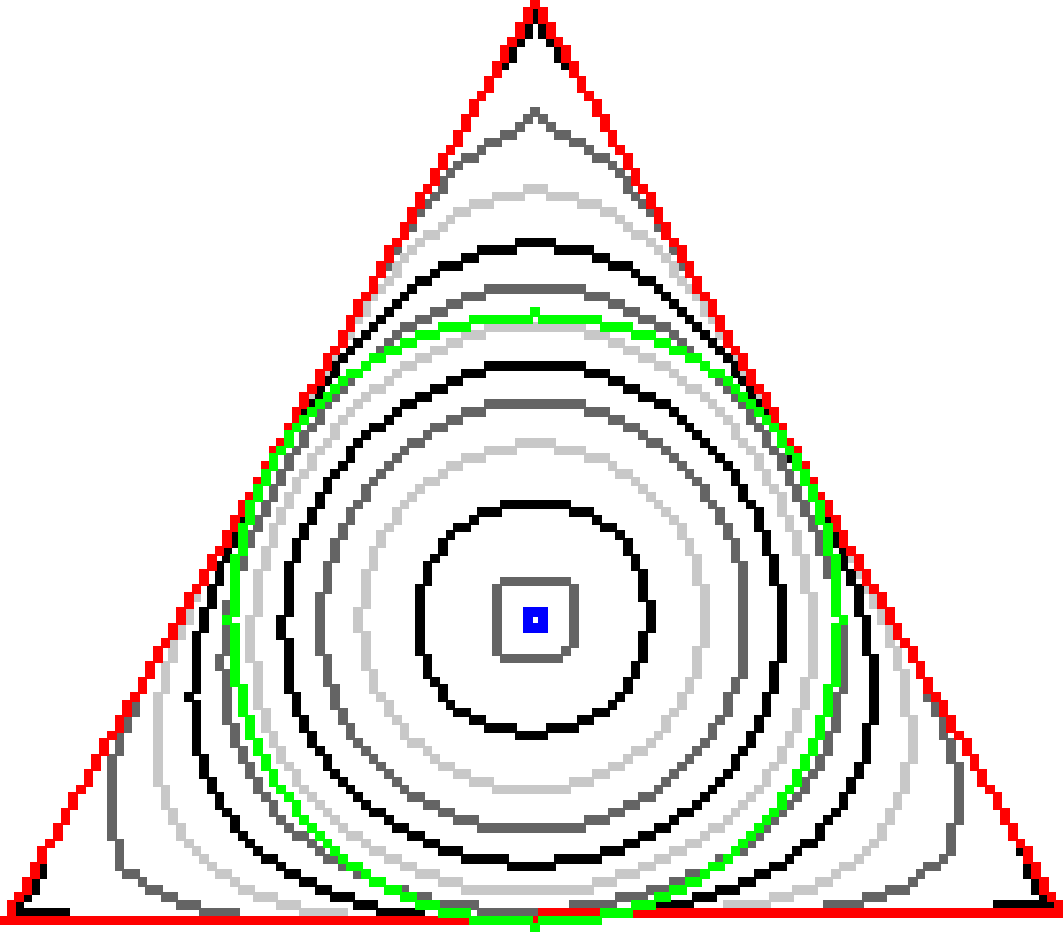
\includegraphics[scale=0.20]{figures/triangle/neigh-0/alpha-0.01/summary.pdf} & 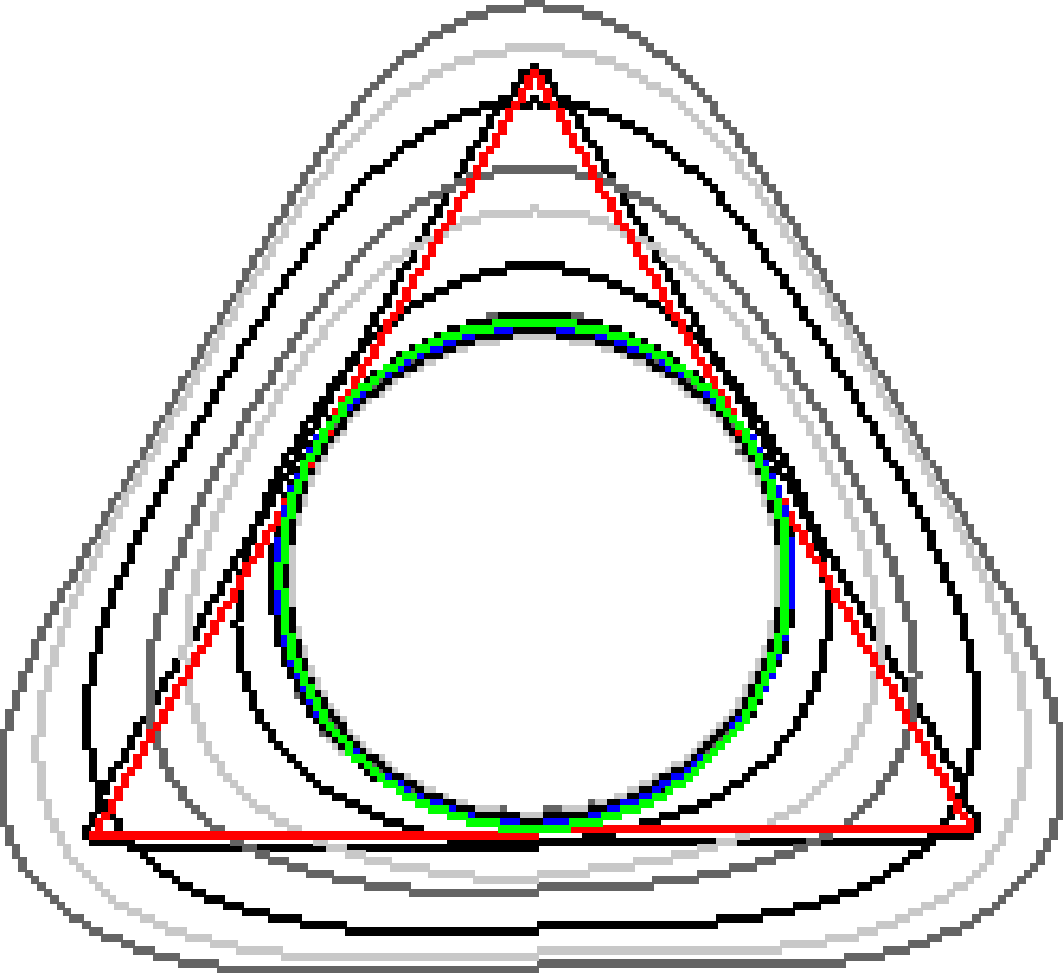
\includegraphics[scale=0.20]{figures/triangle/neigh-2/alpha-0.01/summary.pdf} & 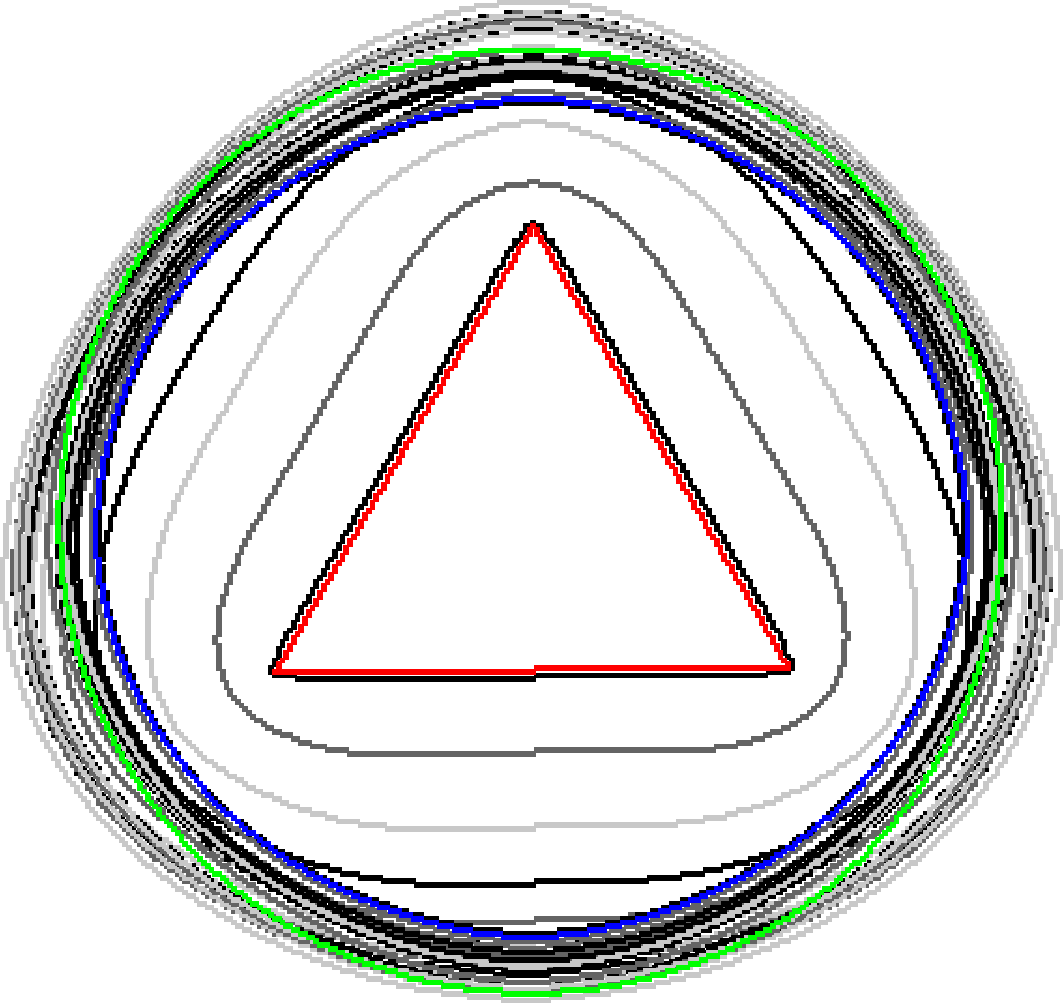
\includegraphics[scale=0.20]{figures/triangle/neigh-2/alpha-0.001/summary.pdf}\\
$(n=2, a=0,\alpha=0.01)$ & $(n=2, a=2,\alpha=0.01)$ & $(n=2, a=2, \alpha=0.001)$
\end{tabular}}
\caption{\textbf{GraphFlow results.} The GraphFlow algorithm can shrink and grow in accordance with length penalization
  and it converges to a shape close to the theoretical global optimum (green curve) in the free elastica problem. We are using $n=2,a=2$ and shapes are displayed every $10$ iterations.\label{ch8:fig:graph-flow-neigh2-results}}
\end{figure}


\begin{figure}
\center
\begin{tabular}{cccc}
\multirow{2}{*}{Seeds} & \multirow{2}{*}{Graph cut} & $\alpha=0.05, \boldsymbol{\beta=0},$ & $\alpha=0.05, \boldsymbol{\beta=0.5},$\\
& & $\gamma_r=\gamma_b=1.0$ & $\gamma_r=\gamma_b=1.0$\\
 	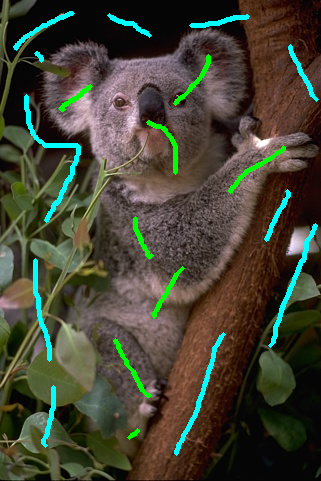
\includegraphics[scale=0.25]{figures/segmentation/coala/k-0.0/seeds.png} & 
 	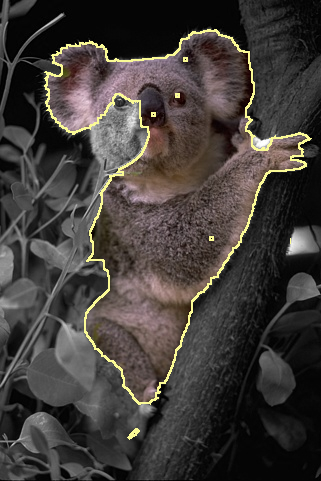
\includegraphics[scale=0.25]{figures/segmentation/coala/k-0.0/gc-seg.png} &  	
 	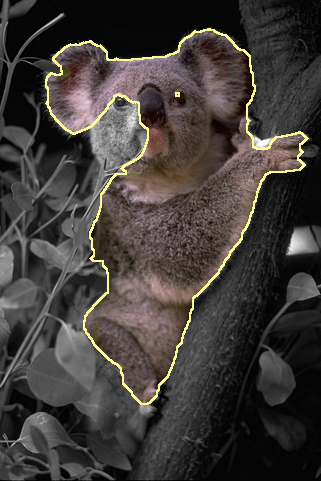
\includegraphics[scale=0.25]{figures/segmentation/coala/k-0.0/corrected-seg.png} &  	
 	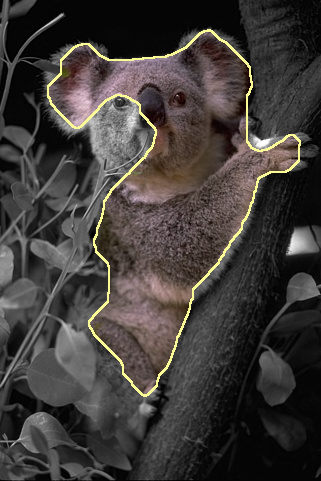
\includegraphics[scale=0.25]{figures/segmentation/coala/k-0.5/corrected-seg.png}
\end{tabular}	
\caption{\textbf{GraphFlow segmentation.} Given foreground (green) and background (gray) seeds in picture (a); Graph cut
  produces picture (b) which is used as input of the GraphFlow algorithm; in pictures (c) and (d) we display the output
  of our Elastica GraphFlow algorithm with and without the squared curvature term in the regularization. }
\label{ch8:fig:segmentation}
\end{figure}

\begin{figure}
\center
\begin{tabular}{cc}
$\alpha=0, \boldsymbol{\beta=0}$ & $\alpha=0, \boldsymbol{\beta=1}$\\
$\gamma_r = 3, \gamma_b = 3$ & $\gamma_r = 3, \gamma_b = 3$\\
 	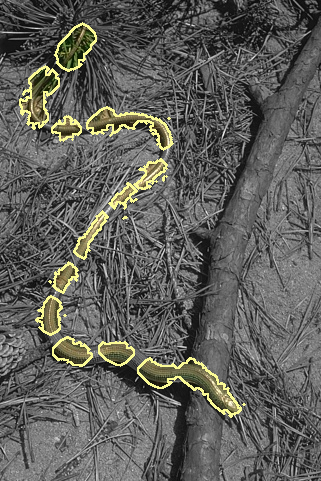
\includegraphics[scale=0.35]{figures/completion/graphseg/alpha-0.0/beta-0.0/gamma-3.0/radius-7/corrected-seg.png} & 
 	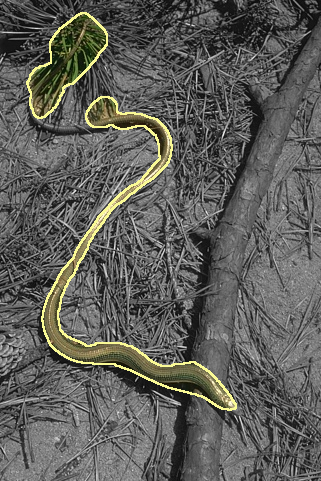
\includegraphics[scale=0.35]{figures/completion/graphseg/alpha-0.0/beta-1.0/gamma-3.0/radius-7/corrected-seg.png}
\end{tabular}	
\caption{\textbf{GraphFlow and completion property}. The oversegmented picture on the left was obtained with no squared curvature regularization, while the picture on the right was obtained by setting $\beta=1.0$. }
\label{ch8:fig:segmentation-curvature-completion}
\end{figure}

The solutions are very similar to those achieved in~\cite{antunes2020elastica}, but with the advantage of producing
smoother flows and up to $100 \times$ faster.  In Fig.~\ref{ch8:fig:segmentation}, we show that our algorithm can easily
be used for segmentation, and that it produces results that are parametrically smoother than those of the BJ model.

In Fig.~\ref{ch8:fig:segmentation-curvature-completion}, we can observe that the Elastica GraphFlow presents the completion
property, i.e., it tends to return a segmentation with fewer disconnected components.

\subsection{Comparisons}
In this section we compare our proposed results for segmentation with several state-of-the-art results in
Fig~\ref{ch9:fig:exp-comparison-image-segmentation-1}: the reference BJ segmentation method; the linear relaxation
methods by Schoeneman \emph{et al.}; and our previous results.

\begin{figure}
	\centering
	\setlength{\tabcolsep}{1pt}
	\begin{tabular}{m{0.25cm}ccc}
          \rotatebox{90}{Graph cut~\cite{boykov01graphcut}} & 
	\figTable{0.25}{\segComparisonFF{flipseg}{airplane}/gc-seg.png} & 
	\figTable{0.25}{\segComparisonFF{flipseg}{kite-surf}/gc-seg.png} & 
	\figTable{0.25}{\segComparisonFF{flipseg}{mans-music}/gc-seg.png} \\[6em]
	
	\rotatebox{90}{SCLR~\cite{schoenemann09linear}} & 
	\figTable{0.25}{\segComparisonScho{schoenemann}{airplane}/airplane.png} & 
	\figTable{0.25}{\segComparisonScho{schoenemann}{kite-surf}/kite-surf.png} & 
	\figTable{0.25}{\segComparisonScho{schoenemann}{mans-music}/mans-music.png}\\[6em]
	
	\rotatebox{90}{Previous work~\cite{antunes2020elastica}} & 
	\figTable{0.25}{\segComparisonFF{flipseg}{airplane}/corrected-seg.png} & 
	\figTable{0.25}{\segComparisonFF{flipseg}{kite-surf}/corrected-seg.png} & 
	\figTable{0.25}{\segComparisonFF{flipseg}{mans-music}/corrected-seg.png} \\[6em]
		
	\rotatebox{90}{GraphFlow (proposed)} & 
	\figTable{0.25}{\segComparisonGF{graphseg}{airplane}/corrected-seg.png} & 
	\figTable{0.25}{\segComparisonGF{graphseg}{kite-surf}/corrected-seg.png} & 
	\figTable{0.25}{\segComparisonGF{graphseg}{mans-music}/corrected-seg.png}
	\end{tabular}
	\caption{\textbf{Segmentation results comparison. Top row, Graph-Cut BJ results; second row: references SCLR
            results; third row: previous results from~\cite{antunes2020elastica}; last row: proposed method. }}
	\label{ch9:fig:exp-comparison-image-segmentation-1}
      \end{figure}

 We observe that our results are smoother than BJ, as in the previous figure. They are very similar to our previous
 results, and much better than the reference SCLR method from literature.

\begin{table}
  \centering
 \caption{Running time for the image segmentation problem.}
\label{ch9:tab:rtime-image-segmentation-general} 
\captionsetup{type=table}
\begin{tabular}{|c|c|c|c|}
\hline
\multicolumn{4}{|c|}{Exp-Comparison Running time}\\
\hline
Model & Minimum & Maximum & Average \\
\hline
SLCR & 2.87min & 52.24min & 18.4min\\
Previous work & 60s & 297s & 156s\\
This work  & 11s & 150s & 75s\\
\hline
\end{tabular}
\end{table}

According to Table~\ref{ch9:tab:rtime-image-segmentation-general}, our proposed method is signifiantly faster than
our previous work, and much faster than the reference SLCR method.

\section{Conclusion}
In this article, we described a graph cut model for optimizing the Elastica energy that is suitable for both discrete curve evolution and
image segmentation. The evolution produced by the Elastica GraphFlow responds to the length penalization term $\alpha$,
i.e., the shape tends to grow (shrink) for lower (higher) values of $\alpha$ and we observe a convergence to a shape
that appears close to the expected, theoretical global optimum in the cases where this globally optimal curve can be
computed. Our Elastica GraphFlow algorithm is significantly faster and simpler to implement than the previous models
presented in the literature.

In our method, we need to use a family of shapes ($a$-probes). In future work, we plan to use a dynamic family with the
help a parameter-free estimator. In the same vein, a multi-resolution approach would be very useful, in particular for
dealing with very thin portions of the image. We also note that a globally optimal solution with multigrid convergent
estimators is yet to be proposed. 

\bibliographystyle{splncs04}
\bibliography{discrete_elastica_dgmm_2021}

\end{document}



%%% the rest below is for reference

\subsubsection{Sample Heading (Third Level)} Only two levels of
headings should be numbered. Lower level headings remain unnumbered;
they are formatted as run-in headings.

\paragraph{Sample Heading (Fourth Level)}
The contribution should contain no more than four levels of
headings. Table~\ref{tab1} gives a summary of all heading levels.

\begin{table}
\caption{Table captions should be placed above the
tables.}\label{tab1}
\begin{tabular}{|l|l|l|}
\hline
Heading level &  Example & Font size and style\\
\hline
Title (centered) &  {\Large\bfseries Lecture Notes} & 14 point, bold\\
1st-level heading &  {\large\bfseries 1 Introduction} & 12 point, bold\\
2nd-level heading & {\bfseries 2.1 Printing Area} & 10 point, bold\\
3rd-level heading & {\bfseries Run-in Heading in Bold.} Text follows & 10 point, bold\\
4th-level heading & {\itshape Lowest Level Heading.} Text follows & 10 point, italic\\
\hline
\end{tabular}
\end{table}


\noindent Displayed equations are centered and set on a separate
line.
\begin{equation}
x + y = z
\end{equation}
Please try to avoid rasterized images for line-art diagrams and
schemas. Whenever possible, use vector graphics instead (see
Fig.~\ref{fig1}).

\begin{figure}
\includegraphics[width=\textwidth]{fig1.eps}
\caption{A figure caption is always placed below the illustration.
Please note that short captions are centered, while long ones are
justified by the macro package automatically.} \label{fig1}
\end{figure}

\begin{theorem}
This is a sample theorem. The run-in heading is set in bold, while
the following text appears in italics. Definitions, lemmas,
propositions, and corollaries are styled the same way.
\end{theorem}
%
% the environments 'definition', 'lemma', 'proposition', 'corollary',
% 'remark', and 'example' are defined in the LLNCS documentclass as well.
%
\begin{proof}
Proofs, examples, and remarks have the initial word in italics,
while the following text appears in normal font.
\end{proof}
For citations of references, we prefer the use of square brackets
and consecutive numbers. Citations using labels or the author/year
convention are also acceptable. The following bibliography provides
a sample reference list with entries for journal
articles~\cite{ref_article1}, an LNCS chapter~\cite{ref_lncs1}, a
book~\cite{ref_book1}, proceedings without editors~\cite{ref_proc1},
and a homepage~\cite{ref_url1}. Multiple citations are grouped
\cite{ref_article1,ref_lncs1,ref_book1},
\cite{ref_article1,ref_book1,ref_proc1,ref_url1}.
%
% ---- Bibliography ----
%
% BibTeX users should specify bibliography style 'splncs04'.
% References will then be sorted and formatted in the correct style.
%
\bibliographystyle{splncs04}
\bibliography{discrete_elastica_dgmm_2021}

\end{document}
